\documentclass[12pt,oneside,a4]{article}
\usepackage{float}
\usepackage[utf8]{inputenc}
\usepackage[a4paper,width=160mm,top=25mm,bottom=25mm]{geometry}
\usepackage[lining,tabular]{fbb} % so math uses tabular lining figures
\usepackage{graphicx}
\usepackage{verbatim}
\usepackage{enumitem}
\setlist{leftmargin=*}
\usepackage{listings}
\lstset{basicstyle=\ttfamily,frame=single,xleftmargin=3em,xrightmargin=3em}
\usepackage[os=win]{menukeys}
\renewmenumacro{\keys}[+]{shadowedroundedkeys}
\usepackage{framed}
\usepackage{etoolbox}
\AtBeginEnvironment{leftbar}{\sffamily\small}
\usepackage{array,lipsum}
\newenvironment{fulltable}[1][H]
 {\begin{table}[#1]%
  \hspace*{-\leftmarginwidth}%
  \begin{minipage}{\fullwidth}}
 {\end{minipage}\end{table}}
\usetikzlibrary{chains,arrows,shapes,positioning}
\usepackage{hyperref}
\graphicspath{{figures/}} %Setting the graphicspath
\renewcommand\abstractname{Introduction}




\title{BANCO : an operational guide\\ \small{v. June 2023}}
\author{CEA/DPhN&DEDIP}
\vspace{3pt}
\begin{document}

\maketitle
\begin{center}
\includegraphics[width=1\linewidth]{figures/BANCO.png}
\end{center}
\begin{abstract}
%\includegraphics[width=1.0\linewidth]{BANCO.png}\\
BANCO is a telescope based on the ALPIDE technology from the MFT detector in ALICE. It allows to recreate the track of a particle, in order to characterise other detectors. The electronics (MOSAIC boards) and the code are based on the test beams for the MFT. This is a document to sum up the setup, the functionalities and few useful results. The goal is to gather all the pieces of information about the different parts of the device. 
\end{abstract}

\clearpage
\tableofcontents

\clearpage
\section{Motivation and Main characteristics}
BANCO was firstly designed to get a simple system to characterise the spatial resolution of other detectors. The idea was to have an easy to use and a transportable device, to carry it in different data taking places.

\bigskip

The main characteristics  of the device are :
\begin{itemize}
    \item 2 arms of 2 ladders to be place close or separately (one at the beginning of the beam, the other at the end).
    \item Acquisition system with or without an external triggering device.
    \item Recreation of tracks and data clustering.
    \item A cooling system to ensure the best temperature conditions for the chips.
\end{itemize}

\begin{figure}[h]
    \centering
        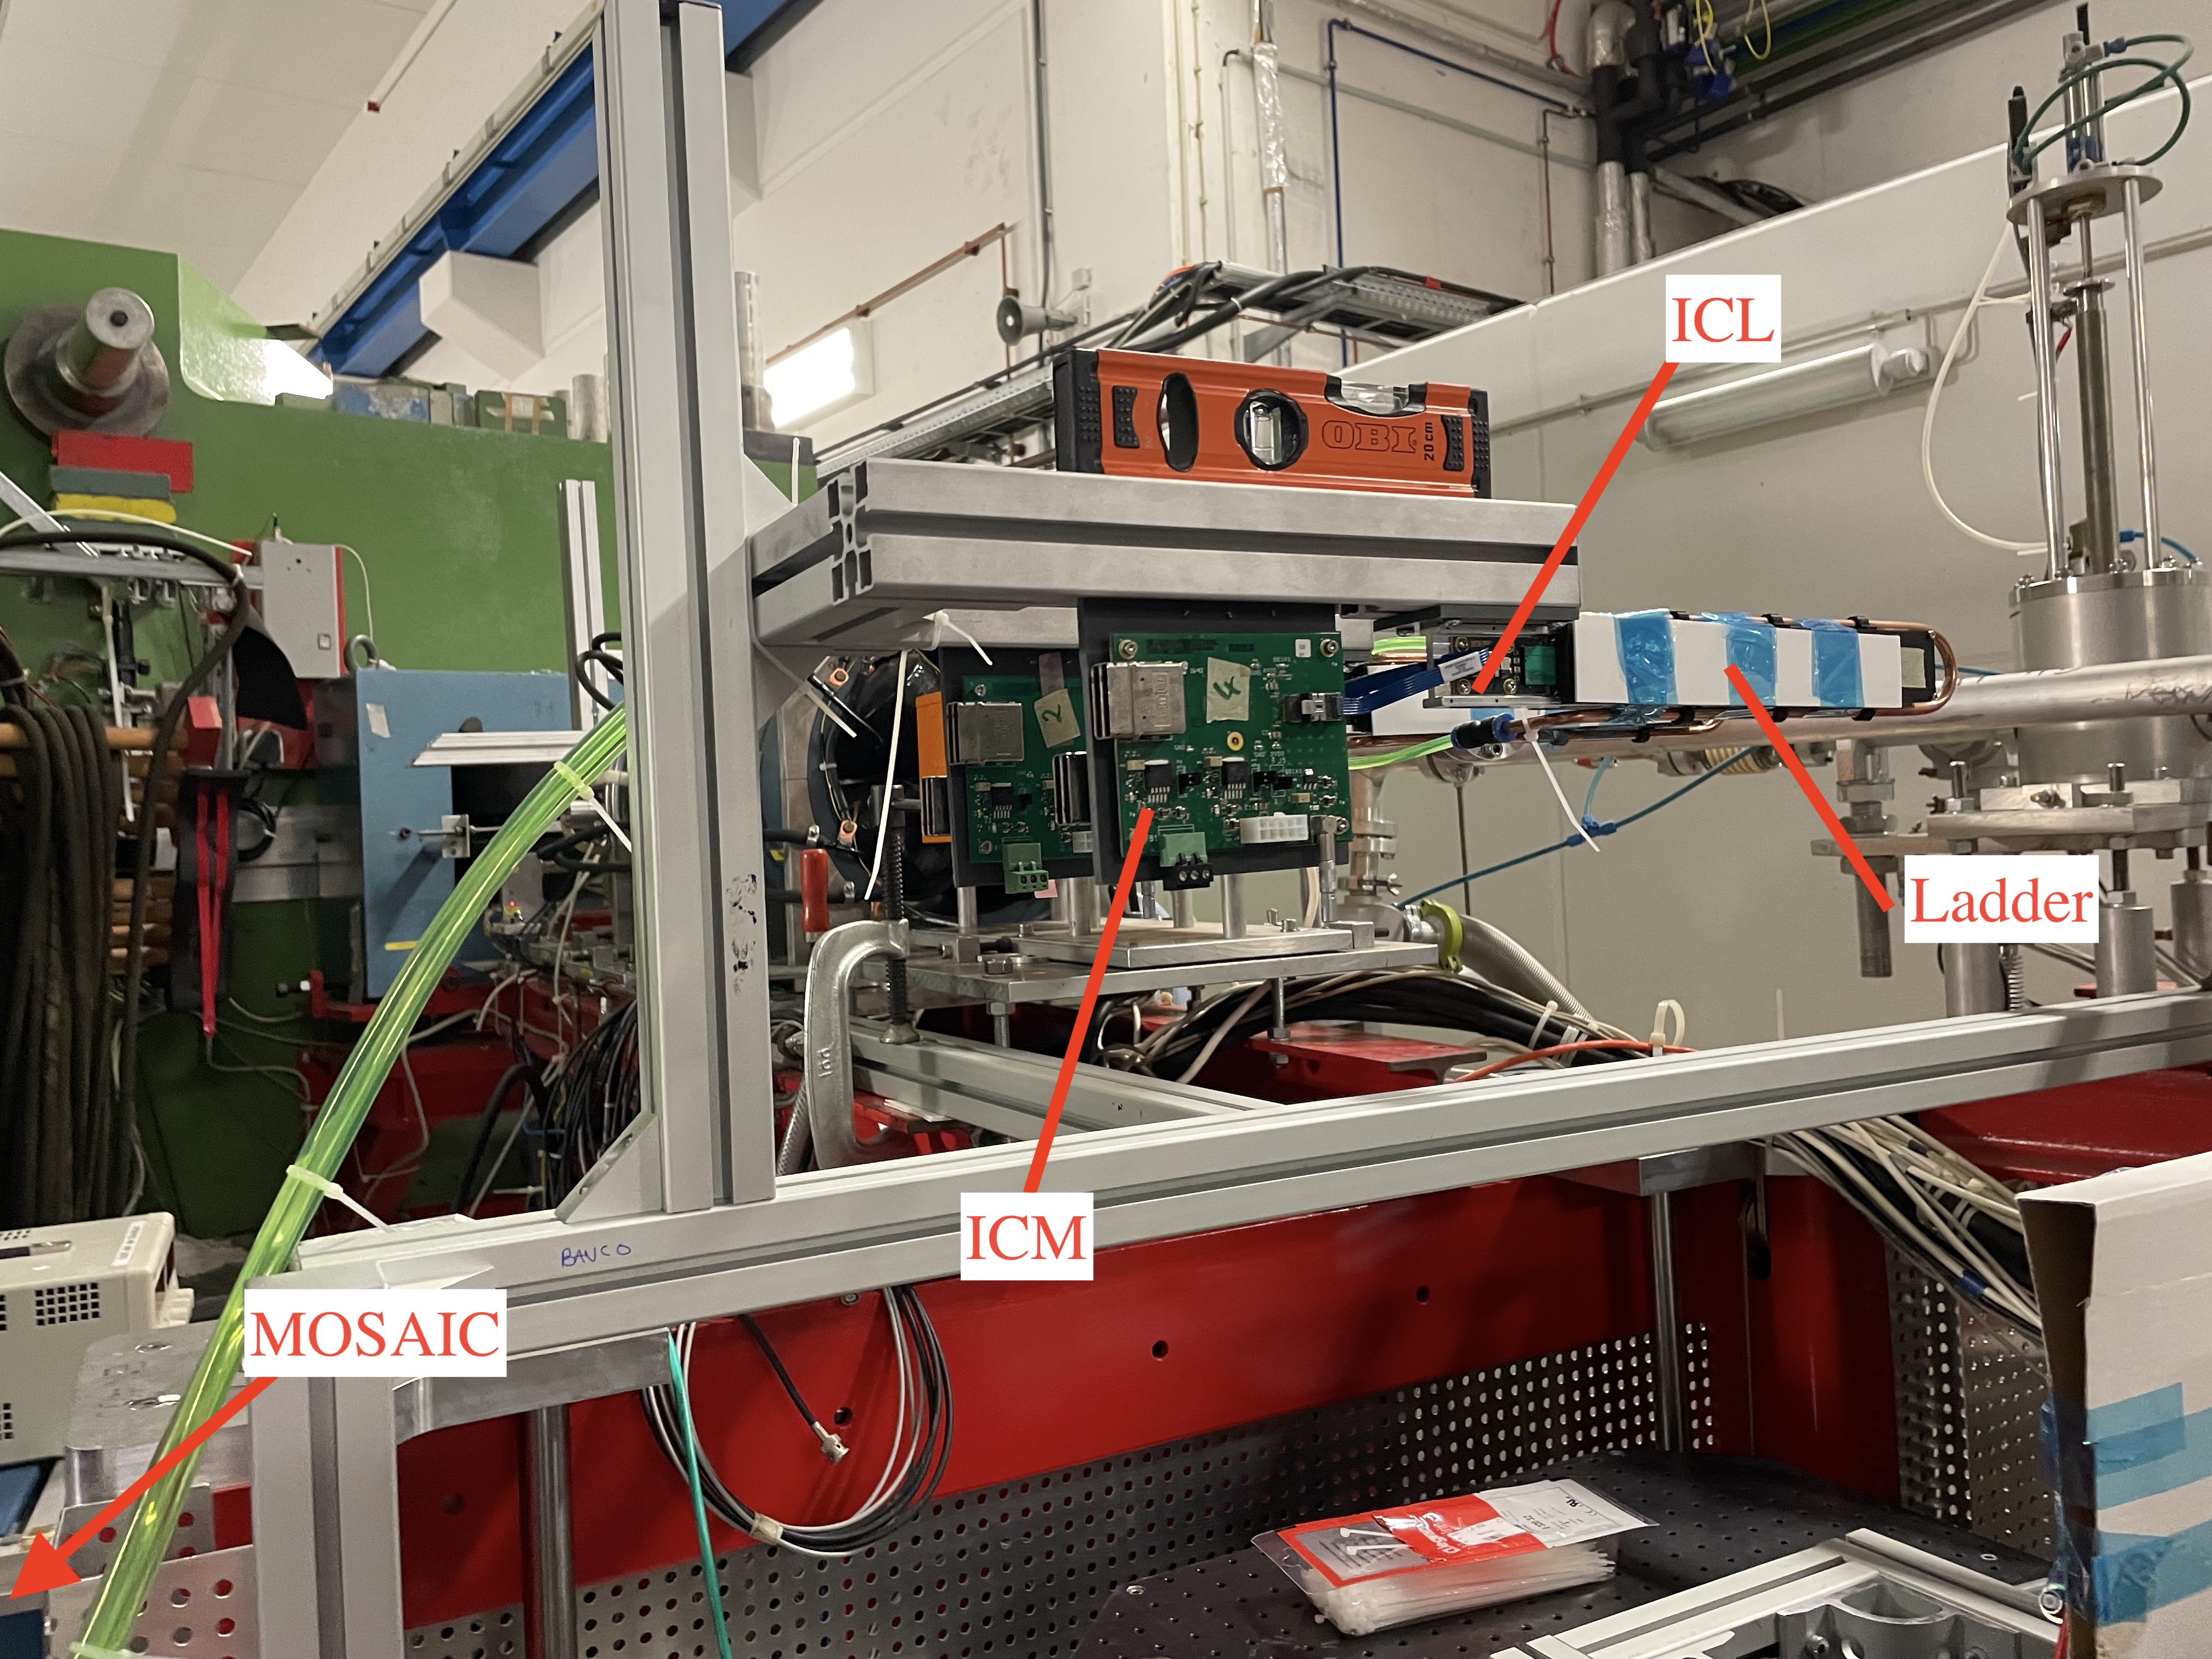
\includegraphics[scale =0.08]{figures/BANCO overview.jpg}
        \caption{Picture of one arm of the BANCO system, with it dedicated electronic}
        \label{fig:2}
    \end{figure}
    
\section{Overview to BANCO }
    \subsection{Mechanics}
    
    One arm of the BANCO detector is composed of an aluminium frame, in which a bonding of 2 ladders, carbon and rohacell (see \ref{fig:1})  is inserted. This allows a minimum 
    material budget and a good thermal conduction. 
    
    \begin{figure}[h]
        \centering
        
\includegraphics[scale =0.5]{figures/BANCO SIDE VIWE.png}
        \caption{Side view of one arm of the BANCO telescope.}
        \label{fig:1}
    \end{figure}
    
    Then, the chips are protected from the light by a plastic cover with a mylar window over the chip, which is screwed on the aluminium frame. 
    
    
    \subsection{Cooling}
    BANCO is equipped with a water cooling system running all around the frame, that has to be connected before any electronic wiring. The system is composed of two electric pumps for each arm of BANCO. It has to be plugged in the copper circuit running around the aluminium. Then, the pumps have to be refill with water and an UV-sensitive liquid that help to detect leaks. 
    To refill the pump, one has to open the upper hole in the pump, and insert liquid in it. Be careful to avoid bubbles in the circuit, or the pump will not run correctly. On the pump, there is a display of the water temperature, and two potentiometers on the card allow to set up the fan and pump speed.

    
    \subsection{Electronics}
        \subsubsection{The ALPIDE}
    The whole telescope is based on the ALPIDE chips which are silcium detectors with in-pixel front end electronics. On each ladder, there are 5 chips, with a size of $15\times30mm$ and a matrix of $512\times1024$ pixels.

    The in pixel circuitry (see \ref{fig:3}, allows the digitization of the signal and store it in a three event buffer, and the user can input signals to test the pixel as well as setup values for the threshold, or the strobe delay and duration (see \ref{Qualification}). 

    \begin{figure}[h]
        \centering
        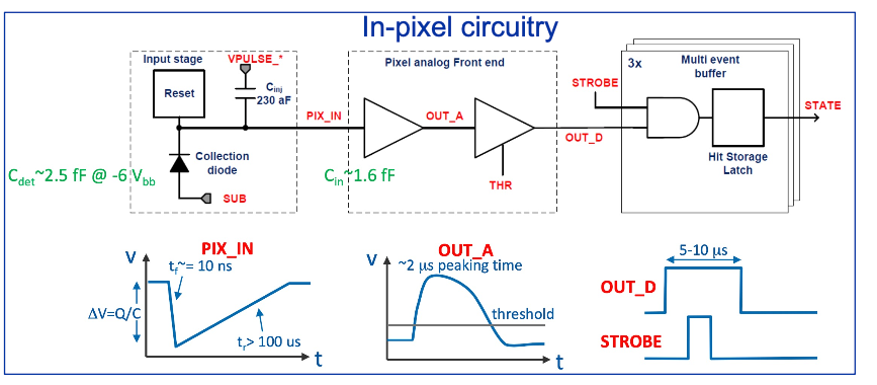
\includegraphics[scale =0.7]{figures/In-pixel circuitry.png}
        \caption{In-pixel circuitry, source : \cite{Alpide}}
        \label{fig:3}
    \end{figure}
    
    As seen on \ref{fig:3}, a particle creates an analogical pulse which is then converted thanks to a threshold discriminator to a logic signal, which is store in the buffer when the STROBE signal and the OUTD signal are high. Thus, the ALPIDE chip can be set in a triggered mode or a continuous mode. On the first case, the Strobe signal is on after the reception of a trigger, whereas in continuous the strobe signal is synchronised with a clock (see chronogram \ref{fig:4}).

    \begin{figure}[h]
        \centering
        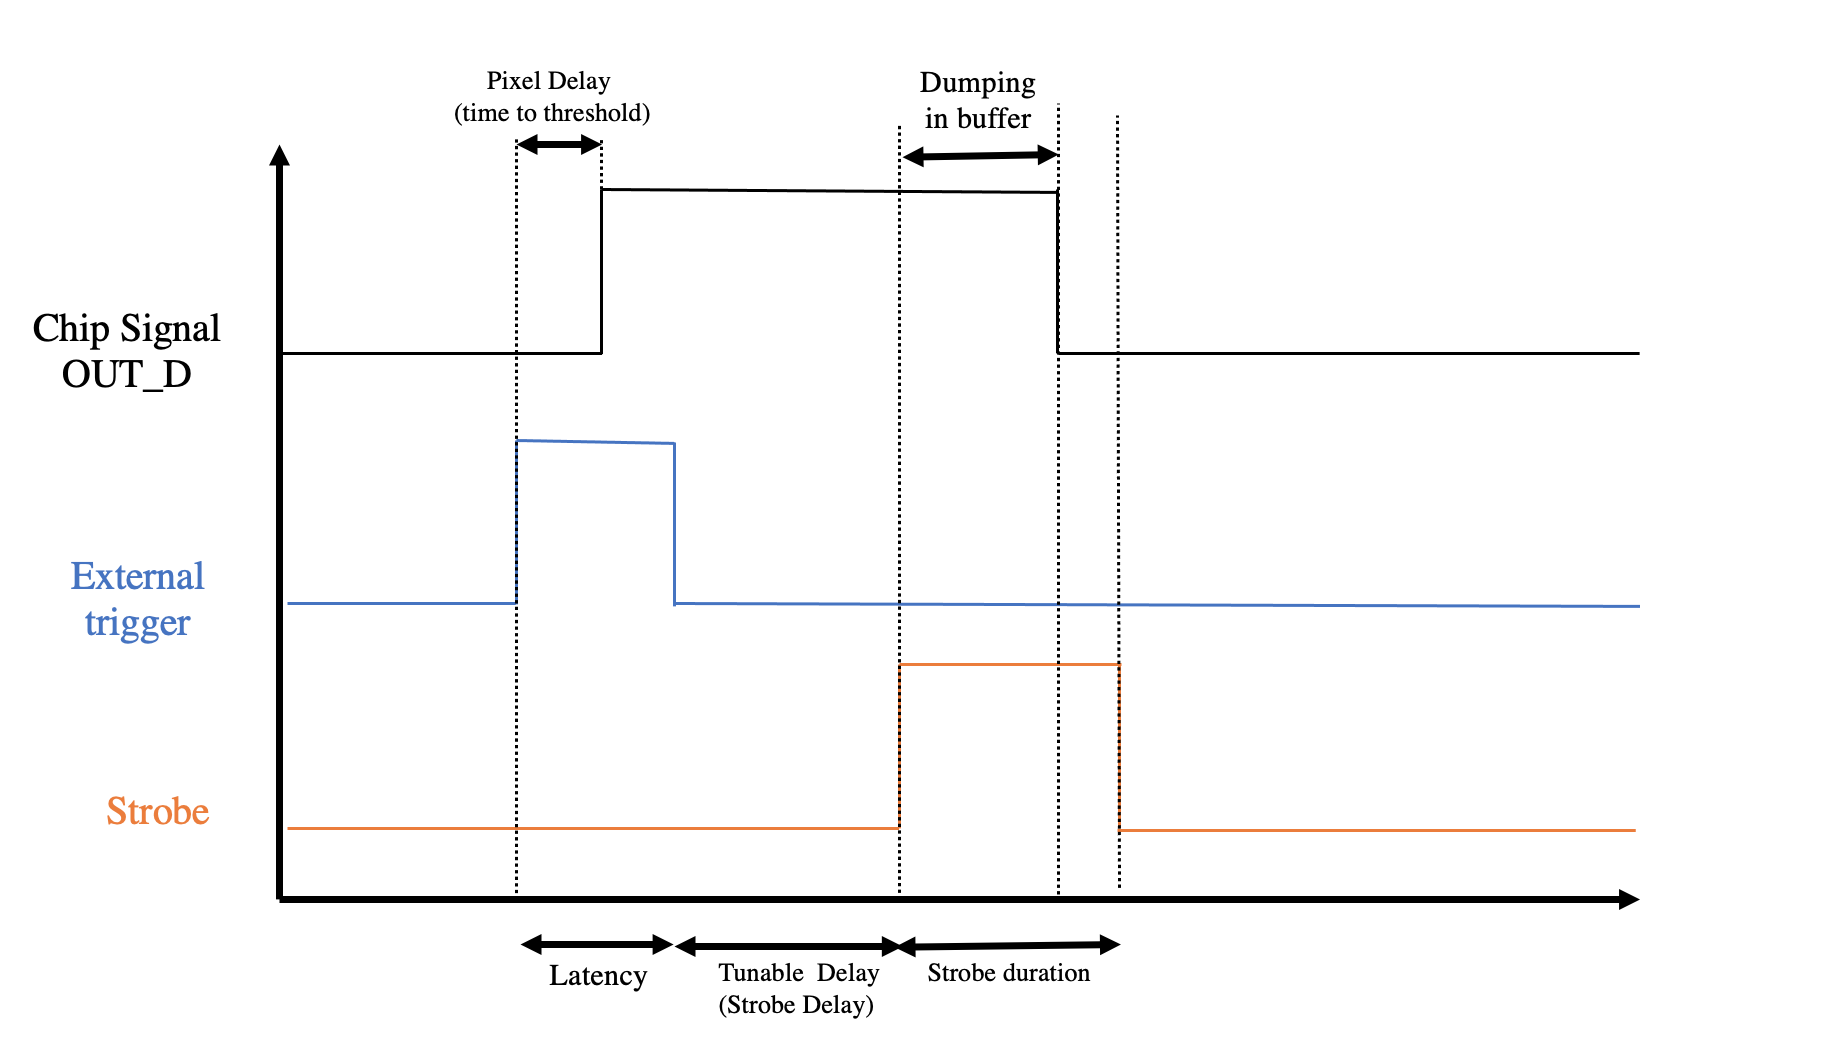
\includegraphics[scale =0.5]{figures/ALPIDE Chronogram.png}
        \caption{Chronogram of the ALPIDE chip}
        \label{fig:4}
    \end{figure}

    
        \subsubsection{The MOSAIC Board}
    The MOSAIC boards are the DAC system associated with the BANCO telescope, for each ladder there is an intermediate card (ICL ) which is linked to another intermediate card (ICM, which mostly enables the power supply), and then to the MOSAIC board (one for each ladder), (see \ref{fig:2}). The MOSAICs are configured in a Master/Slave mode : the trigger and the clock are sent to the slaves by the Master and then all the MOSAICs are sending their busy to the external trigger if it's working with another system (See each config \ref{fig:5})

Each MOSAIC board has an unique IP address, in order to communicate with the computer used for the acquisition. There is a config file for each ladder and so each MOSAIC board, to set up those addresses and their role in the acquisition. Furthermore, the config file enables the acquisition to be on an internal constant trigger (1MHz) or depending on an external trigger.

\subsubsection{With an external system}
The main goal of the BANCO system is to be synchronized with other acquisition system. To do so, the BANCO system has to send back a common busy to the triggering system. Here is an overview of the logic used :
\begin{figure}[h]
\hspace*{-2cm}
        \centering
        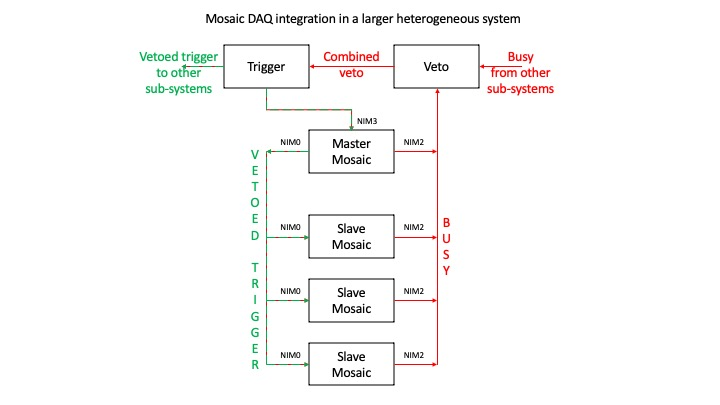
\includegraphics[scale =0.8]{figures/Triggering.jpeg}
        \caption{Triggering system, source : Irakli Mandjavidze}
        \label{fig:8}
\end{figure}


\newpage
\section{Getting started}
    \subsection{Wiring the system}
The wiring of BANCO comes in two parts, first wiring the ladders with their respective MOSAIC boards and the MOSAIC boards with the computer, and then linking the system with the other electronics in a given experiment.
        \subsubsection{Alone}
        \begin{figure}[h]
        \centering
        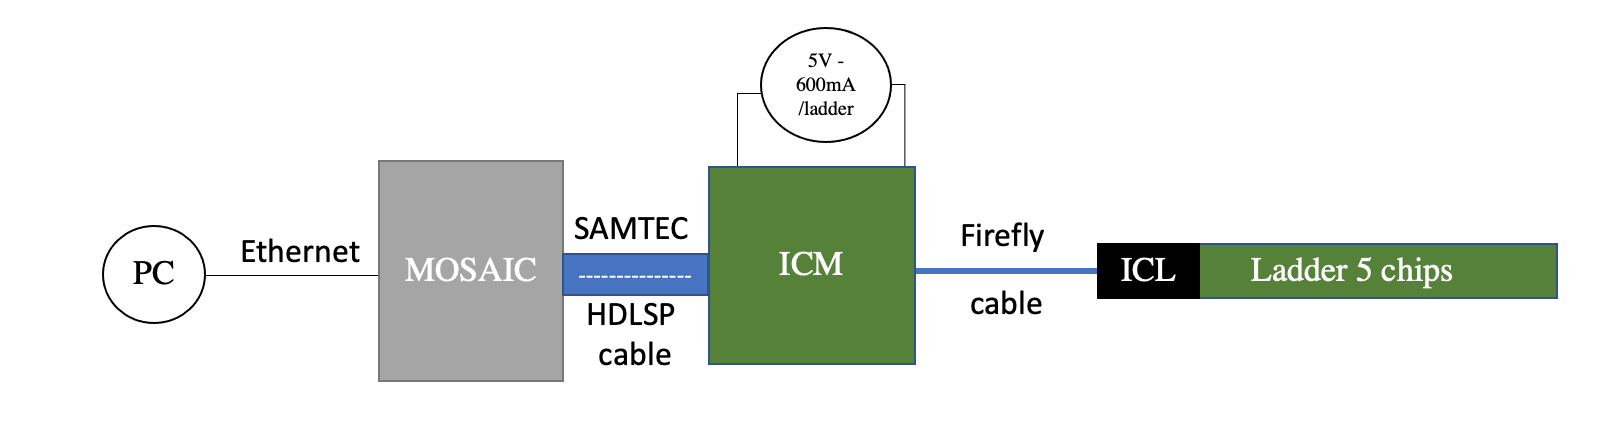
\includegraphics[scale =0.5]{figures/Wiring_ladder.png}
        \caption{Wiring of a ladder}
        \label{fig:6}
    \end{figure}
    
To ensure a good power supply to the ICM, the supply must be connected as on \ref{fig:7}, and te power supply set on 5V and 0,6A per ladder (if two ladders are on the same output put 1,2A). Then, powering on the 5V supply, it is important to check the value of the DVDD, and that the current is at 0,17 A per ladder (if no ongoing test). To do so, place a multimeter on the capacity C5 of the ICL (you can also measure it on the ICM, but there is a voltage drop to take into account). Make sure, it is over 1,83V and below 1,89V, to adjust the value there is a potentiometer on the ICM (see \ref{fig:7})

\begin{figure}[h]
        \centering
        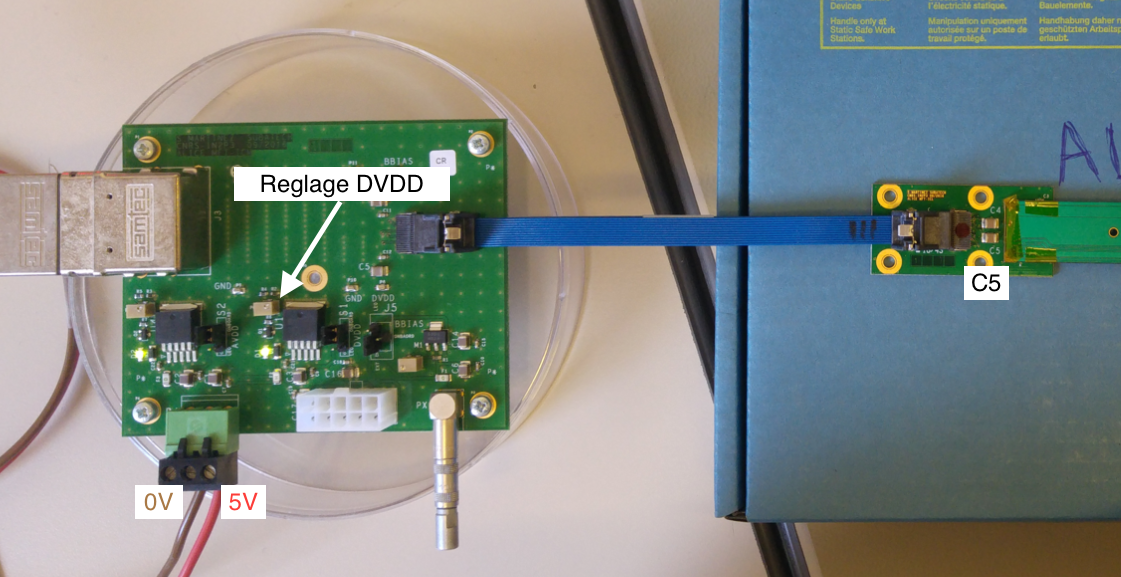
\includegraphics[scale =0.8]{figures/Alimentation.png}
        \caption{Intermediate Cards wiring}
        \label{fig:7}
\end{figure}

Then, power on the cooling system and proceed to the wiring of the MOSAIC boards. To do so, follow the configuration on \ref{fig:5}. This table summarizes the configuration for the IP address of the MOSAIC and the different NIM ports.


        \begin{center}
\begin{figure}[h]

\small
\begin{tabular}{||c c c c c||} 
 \hline
 Ladder : & 1 (162) & 2 (157) & 3 (163) & 4 (160) \\ [0.5ex] 
 \hline\hline
 IP MOSAIC : & 192.168.168.250 & 192.168.168.20 & 192.168.168.30 & 192.168.168.40 \\ 
 \hline
 Function : & Master & Slave & Slave & Slave \\
 \hline
 NIM 0 (Trigger and Clock) : & Out & In & In & In \\
 \hline
 NIM 2 (Busy) : & Out & Out & Out & Out \\
 \hline
 NIM 3 (External Trigger) & In & None & None & None \\ [1ex] 
 \hline
\end{tabular}
   \caption{Table of the ladder and their MOSAIC settings}
    \label{fig:5}
\end{figure}
\end{center}

After all those connections, one can power on the MOSAIC boards and get ready to qualify the system and then make measurements.

\subsection{Qualification}\label{Qualification}
After those different steps of wiring,  each ladder needs to be qualified for the acquisition, especially to tune the values of VCASN and ITHR, that will ensure a threshold of 100 electrons recorded. For this part, we use a first software : the SingleLadderQualification \cite{SingleLadderQualification} (installed on the computer connected to the MOSAIC boards).

A GUI is used to manage the tests, to open it, one should first set the root environment and open the GUI, with the following commands in the shell :

\begin{verbatim}
$setup-o2-root //you will get an error message of two lines, it is normal
$cd SingleLadderQualification/build
$./GUI/GUI
\end{verbatim}


Then, in the GUI, on the top left, one can set up a test (top picture on \ref{fig:9}. Especially, in this case we want to do a threshold tuning, and get the values of ITHR and VCASN for a given ladder.

In the menu for a test (bottom picture \ref{fig:9}, one should input the IP address of the corresponding MOSAIC board,  the number of chips (5) (NB : chips that are not working anymore can be disabled, especially \textbf{on ladder 160 the chip 6 should be disabled}, during the qualification as during an acquisition). Be sure to set the correct Ladder Id according to \ref{fig:5}. Click apply settings. Then a new window will appear, press Load pre-selected settings. 
Then, it will display the different chips on the ladder rather in green or red. If there are any red chip be sure to check all the wiring, if it is only one chip you can basically disable it. 

After the test, the result with the different values (VCASN, ITHR) for each chip of a ladder is in the shell. There are important, and will be used for the measurement as a config input.

There are other tests that can be done to qualify the ladder, it can be useful for debugging combined with the internal note about the soft (see \cite{Note}).

\begin{figure}[h]
        \centering
        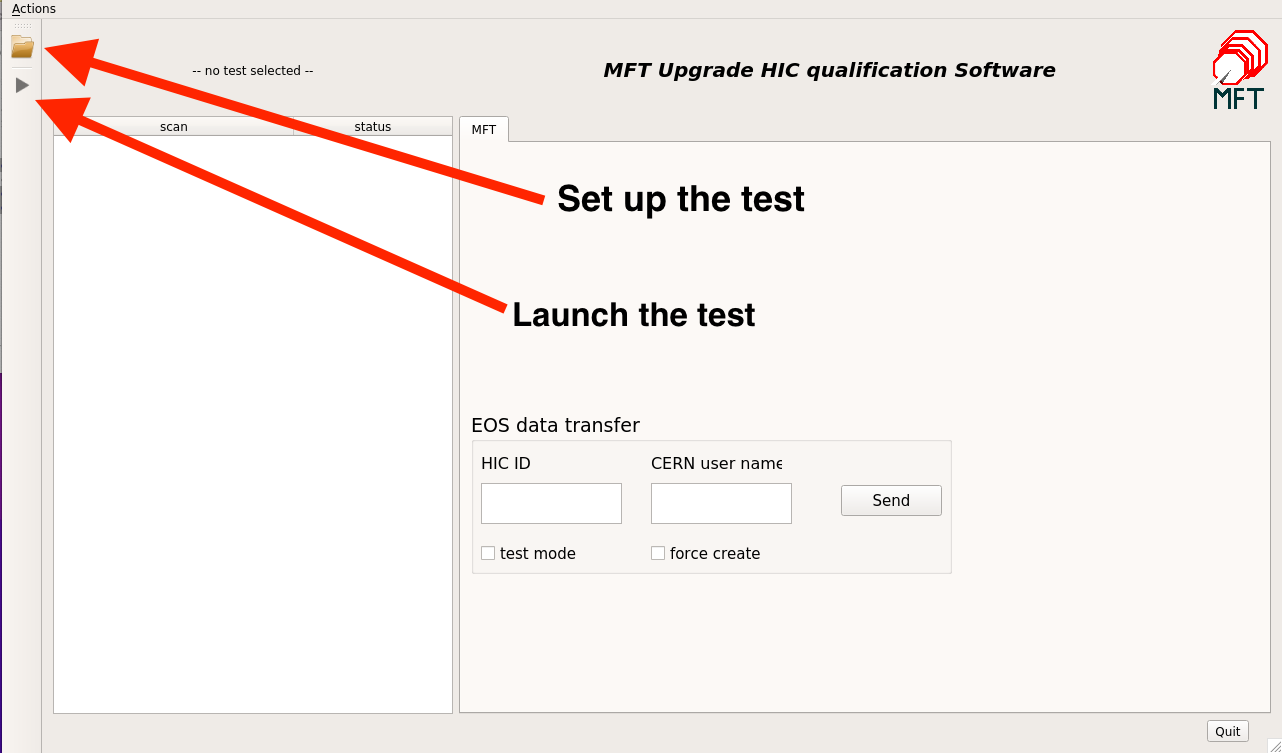
\includegraphics[scale =0.3]{figures/Interface_example_1.png}
        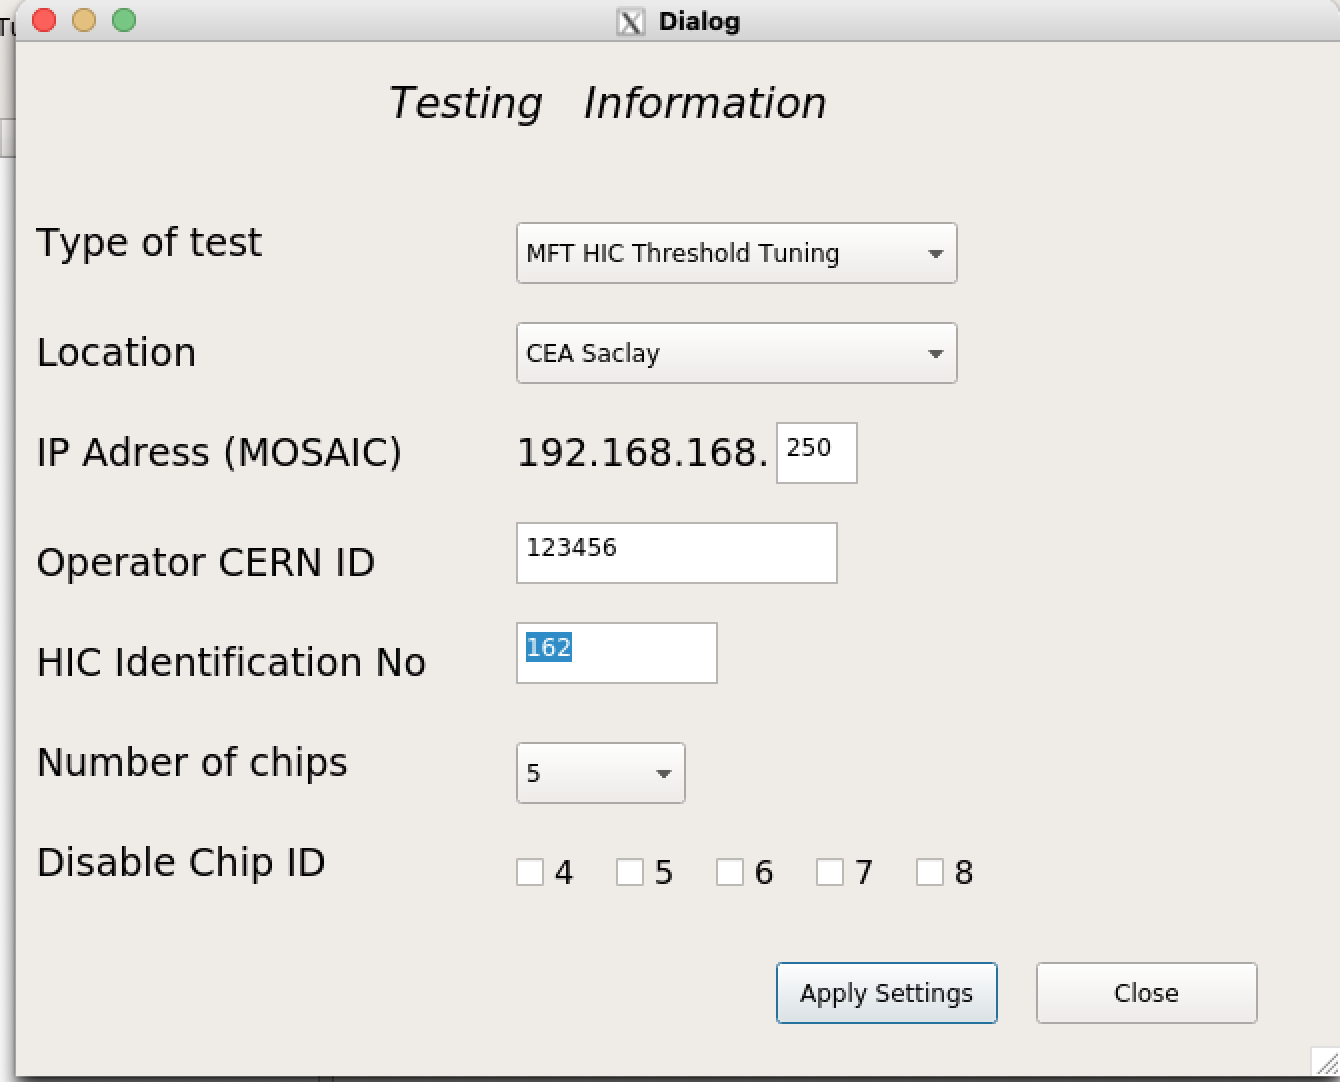
\includegraphics[scale =0.3]{figures/Interface_example_2.png}
        \caption{GUI for qualification ( up : general window, bottom : test settings)}
        \label{fig:9}
\end{figure}

\section{Making Measurements}
    \subsection{Software presentation}
The working repository to make modifications on the program is \textit{MultiLadderOperation}. To do your own measurement, be sure to create a new working directory and to copy the compile executable and the given con fig files as on \ref{fig:14}.

\begin{figure}[h]
        \centering
        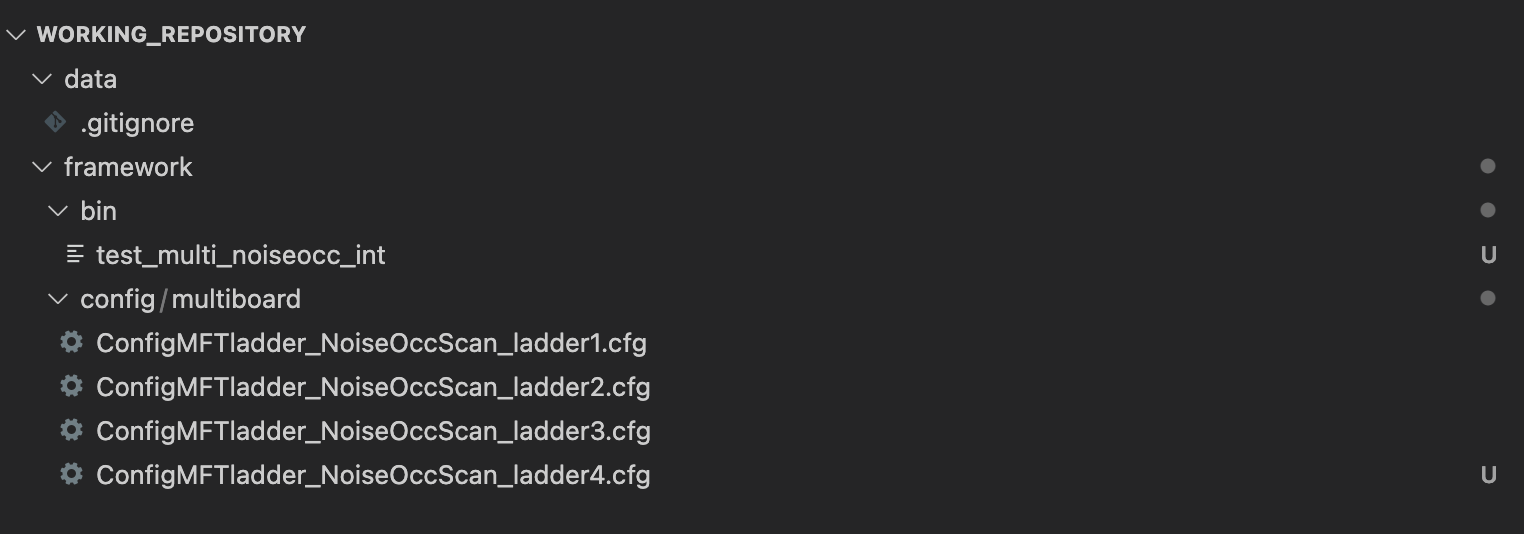
\includegraphics[scale =0.3]{figures/Repository.png}
        \caption{Structure of the working directory}
        \label{fig:9}
\end{figure}

You will then, have to set up the config file, in framework$\rightarrow$config$\rightarrow$multiboard.

 \subsubsection{Config File presentation}\label{Config File presentation}
There is a configuration file for each ladder in BANCO (Test\textunderscore Beam$\rightarrow$framework$\rightarrow$config$\rightarrow$multiboard
$\rightarrow$ConfigMFTladder\textunderscore NoiseOccScan\textunderscore ladderX.cfg). 

\bigskip

They have all the same structure and the main settings are the following (NB : Here the chip labelling is different 0 corresponds to chipId=4 and 4 to chipId=8):
\begin{itemize}
    \item ENABLED\textunderscore 0  (Line 36) : when set to 0 it will disabled a chip. This can be useful to exclude a noisy chip or a non working one. (\textbf{chip 6 on 160}
    \item NTRGPERTRAIN and NTRIGGERS (Line 75,76), this command enables to set the number of triggers before the acquisition end and the number of triggers per train (important for the multi threading).
    \item ADDRESS (Line 88) : the IP address of the MOSAIC see \ref{fig:5}
    \item TRIGGERSOURCE : to set the trigger internal(1) or external (0)
    \item MASTERSLAVEMODEON, MASTERSLAVEMODE, DEVICEID (Line 129-131) : the first is to work in mastersalve mode (1 On 0 Off), the second is to configure the role of the ladder (1 Master 2 Slave) and the last is to set the ID of the ladder.
    \item ITHR, VCASN, VCASN2 (Line 165-180) these parameters are there to set the value of the threshold, it has to be an integer and adding an underscore enables to set the value for a specific chip (ex : ITHR 54\textunderscore 0 fix a value of 54mA on the chip 4 for ITHR)  
\end{itemize}

If you want to remove a ladder from the measurement, it is another procedure to follow. You have to modify the main function in  MultiLadderOperation$\rightarrow$framework$\rightarrow$exe. You want to modify the main\textunderscore multinoiseocc\textunderscore int.cpp. Especially, remove the line of AddSetup corresponding to the ladder you want to remove. 

\subsubsection{Launching a measurement}


\begin{verbatim}
$setup-o2-root
$cd your_working_repository/framework/bin
$./test_multi_noiseocc_int
\end{verbatim}

Then, the program will launch, first with the configuration procedure, which set up the parameters from the config file and get ready to take measurement. Then, the program starts the measurement when the following message is displayed : 
\begin{verbatim}
    TMultiDeviceOperator::GoNoiseOccScan() - nTriggers: ...
    TMultiDeviceOperator::GoNoiseOccScan() - nTriggersPerTrain: ...
    TMultiDeviceOperator::GoNoiseOccScan() - nTrains: ...
    TMultiDeviceOperator::GoNoiseOccScan() - nRest: ...
    TMultiDeviceOperator::GoNoiseOccScan() - trains: ...
\end{verbatim}

Then, the program will launch on the trigger (external or internal). In particular, with an external trigger, one should wait for this message and \textit{Waiting for trigger...}., to start the triggering. 
To end the program, one should wait for the maximum trigger number or kill the process with a CTRL+C, the program will then write the different root files (see \ref{Data overview}).


       
    \subsection{Masking}
A proper masking procedure has yet to be done, but there are two important things to know : the moment to do it and the right register to update. The ideal place to do it, is in \textbf{MultiLadderOperation$\rightarrow$framework$\rightarrow$src$\rightarrow$manager$\rightarrow$TAlpide.cpp} in the fonction BaseConfigMask. And the right code to do so is : 
\begin{verbatim}
    WritePixRegSingle( AlpidePixConfigReg::MASK_ENABLE, true, row, col )
\end{verbatim}
This will enable masking on the pixel in the given row and col, true for masking and false to enable the pixel to be seen again.
\section{Data processing}
    \subsection{Data overview}\label{Data overview}
    After a measurement, the output data is saved in Test\textunderscore Beam$\rightarrow$data. 
    There are a lot of different plots extracted from the measurement, especially there are histograms by ladder and by chips, but the ones we use are the root files by ladder. The typical name of such a file is : \textit{multinoiseScan\textunderscore date\textunderscore hour\textunderscore RUNXX-B0-ladderXXX.root}
    
    The structure of the root file can be seen on \ref{fig:10}. The important elements are the X and Y coordinate. One entry in the tree corresponds to a hit detected on a pixel of coordinates (col,row).
    
\begin{figure}[h]
        \centering
        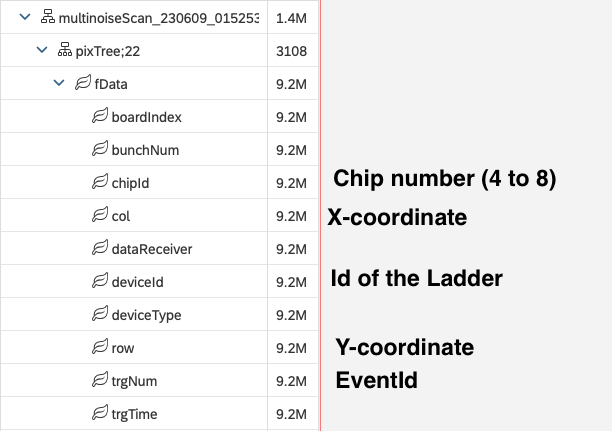
\includegraphics[scale =0.7]{figures/ROOT_file.png}
        \caption{Root tree associate with a ladder}
        \label{fig:10}
\end{figure}

With the definition of the axis as following \ref{fig:11}:

\begin{figure}[h]
        \centering
        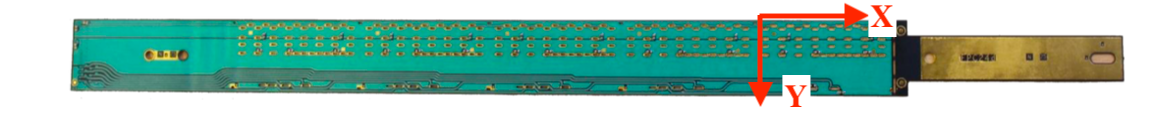
\includegraphics[scale =0.7]{figures/Axis.png}
        \caption{Axis definition}
        \label{fig:11}
\end{figure}

A git \cite{DataVisualisation} is available to visualize those data using Python, of course one can also use root to visualize the data produced. 
In this python code, the coordinates used are the pixels from the ladder, considering the (0,0) coordinate as the (0,0) of the first chip of the first ladder. We have also modified the coordinates from 3 coordinates (chipId, row, col) to 2 (row,col), where $col=col+(chipId-4) \times 1024$. This is to recover a real spatial repartition among all the ladder.
Then, the code (\textit{open\textunderscore file}) will produce a python data frame that can be plotted and displayed as produced in \ref{fig:12}.

\begin{figure}[h]
        \centering
        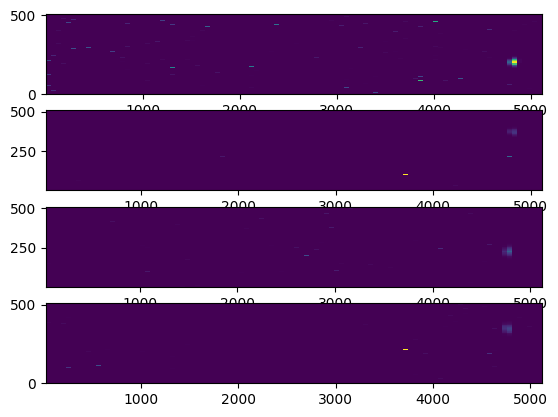
\includegraphics[scale =0.7]{figures/Without_noise removal.png}
        \caption{Raw integrated plotting of RUN73 on the four different ladders (hist2d function)}
        \label{fig:12}
\end{figure}

    \subsection{Noise removal}
    
One can then load a Noise file using \textit{open\textunderscore noise} program, from then it is possible to apply the noise removal filter with the \textit{remove\textunderscore noise} function. And to ensure a more precise analysis one can choose to focus on the hit chip. Here is an example of such a filter \ref{fig:13} :

    \begin{figure}[h]
        \centering
        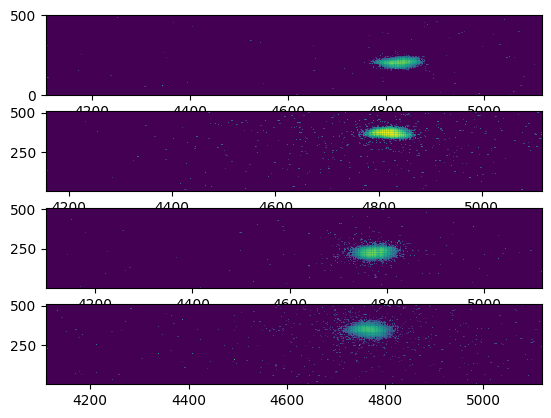
\includegraphics[scale =0.5]{figures/With_noise_removal_and_chip_focus.png}
        \caption{Integrated plotting of RUN73 on the fourth different ladders after noise removal and focused on the hit chip (here chip 8) (hist2d function)}
        \label{fig:13}
    \end{figure}
\newpage
    \subsection{Clustering and Tracking}
    \subsubsection{Clusters}
    In the python program, there are other scripts to do the clustering of the data and reducing the hits to their barycenters. 
    The clustering uses a Density-based spatial clustering with a distance threshold of 1 between two points of a same cluster : the algorithm visits the different point for a given even and if the point has points in its neighbourhood they are added to a same cluster, if not the point will be considered as an isolated point. 
    We try to get an average cluster size of 2 to 2.5 by cluster, and single event (1 cluster 1 event) as often as possible. 
    \subsubsection{Alignement}
    Work in progress
    


\newpage
\begin{thebibliography}{99}
\bibitem{Manual}
ALICE ITS ALPIDE development team (2017), Alpide Operations Manual.
\bibitem{Note}
Lucrezia Camilla Migliorin (2021), Statistical results on ALPIDE sensors of the Muon Forward Tracker during the detector surface commissioning.
\bibitem{Mosaic}
INFN sez Bari, CAD service (2015), MOSAIC User's Manual.
\bibitem{Alpide}
G. Aglieri Rinella, The alpide pixel sensor chip for the upgrade of the alice inner tracking system, Nuclear Instruments and Methods in Physics Research Section A: Accelerators, Spectrometers, Detectors and Associated Equipment 845 (2017) 583.
\bibitem{SingleLadderQualification} SingleLadderQualification Software, \href{https://github.com/AudreyFrancisco/SingleLadderQualification}{GitHub}
\bibitem{DataVisualisation} DataVisualisation Repository,  \href{https://github.com/fbossu/beam_test_2023/tree/Banco/banco}{GitHub}
\end{thebibliography}
\end{document}